\documentclass[TeamE-eindrapport]{subfiles}

\begin{document}
	
	\chapter{Features}
	
	\section{Overzicht}
	
	Zoals in de inleiding reeds vermeld werd, bestaat onze dataset uit een \(500\)-tal datapunten met elk \(30\) features. Hieronder lijsten we de eerste features op om de lezer een idee te geven van de data die voor handen is:
	
	\begin{itemize}
		\item Straal (gemiddelde van afstanden van het middelpunt tot punten op de omtrek)
		\item Textuur (standaardafwijking van grijswaarden)
		\item Omtrek
		\item Oppervlakte
		\item Gladheid (lokale variatie in straallengtes)
		\item Compactheid (\(omtrek^2 / oppervlakte - 1.0\))
		\item Concaafheid (ernst van concave delen van de contour)
		\item Concave punten (aantal concave delen van de contour)
		\item Symmetrie
		\item ...
	\end{itemize}
	
	\section{Limitaties}
	
	Zoals we verder zullen ontdekken in hoofdstuk \ref{tekst:svm}, botsen we tegen een limitatie wat betreft het aantal features die we kunnen gebruiken voor ons model. Indien we het aantal features opdrijven, worden de wiskundige berekeningen namelijk een pak complexer en zouden we dus meer tijd nodig hebben om dit helemaal uit te werken. Daarnaast wordt het visueel voorstellen van de dataset ook des te moeilijker bij een toenemend aantal features. Wegens deze twee limitaties, zullen we ons dus beperken tot slechts twee features per tumor.
		
	\section{Selectie}
	
	Hoe selecteren we nu de twee interessante features? We kunnen daarvoor gebruik maken van een \textit{pairplot}, zoals er een te zien is in figuur \ref{fig:pairplot}. Een \textit{pairplot} is een visuele weergave van de relatie tussen paren van features in een dataset. In machine learning worden dit soort voorstellingen vaak gebruikt om patronen en verbanden tussen de verschillende features van een dataset te identificeren. Op basis van deze pairplot bepaalden wij dat \textit{mean texture} (textuur) en \textit{mean radius} (straal) twee interessante features waren om te bestuderen.
	
	\begin{figure}
		\centering
		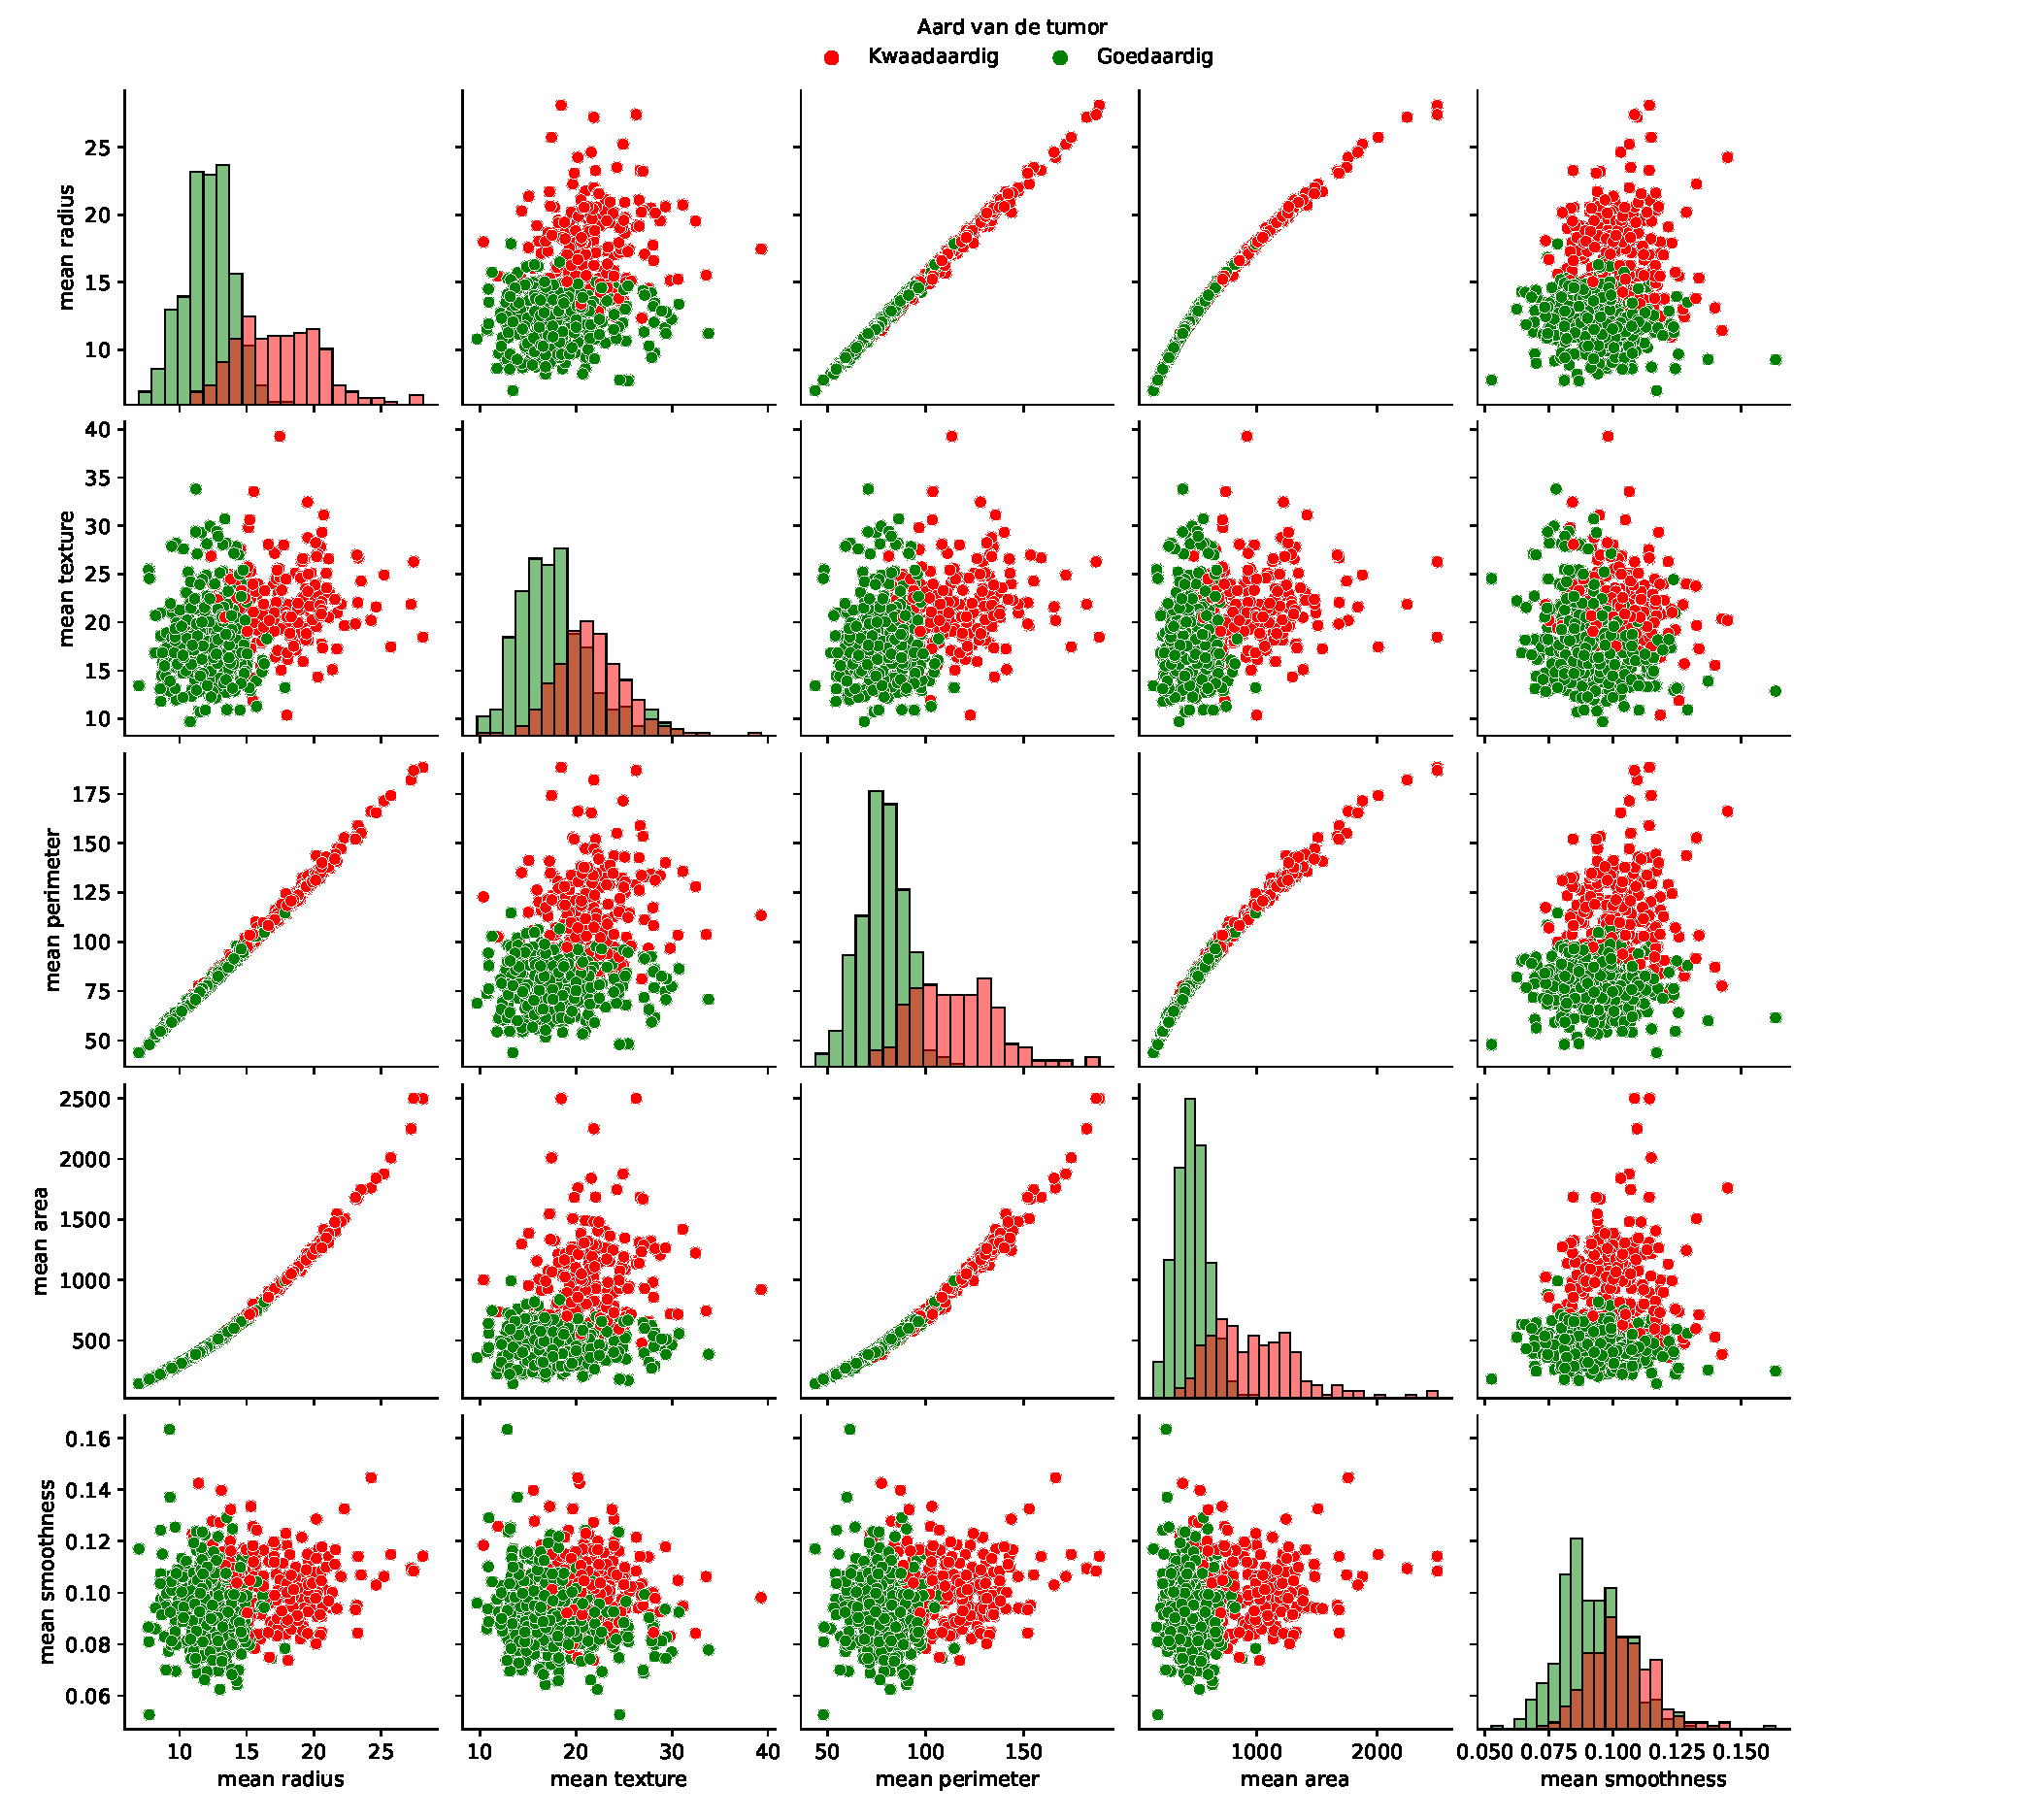
\includegraphics[width=1\textwidth]{pairplot}
		\caption{Een pairplot van de eerste 5 features in de tumordataset.}
		\label{fig:pairplot}
	\end{figure}
\end{document}

